\documentclass{article}

\usepackage{amsmath, graphicx}

\title{Revis\~ao R\'apida de Processos At\^omicos}
\author{Rafael Lopes de S\'a}
\date{\today}

\begin{document}
\maketitle

\section{Efeito fotoel\'etrico}

\subsection{Resumo}

O efeito fotoel\'etrico consiste num el\'etron de um metal absorvendo um f\'oton de forma que esse el\'etron se torna livre:

\begin{equation}
\text{el\'etron ligado} + \text{f\'oton} \rightarrow \text{el\'etron livre}
\end{equation}



Se a energia do f\'oton absorvida pelo el\'etron for maior que a energia de liga\c c\~ao do el\'etron com a estrutura met\'alica, o el\'etron vai se tornar livre e pode formar uma corrente el\'etrica. Quase todo problema sobre efeito fotoel\'etrico se resolve usando conserva\c c\~ao de energia. Conceitualmente:

\begin{equation}
\begin{split}
(\text{energia do f\'oton}) &- (\text{energia gasta para liberar o f\'oton da estrutura met\'alica}) = \\
&(\text{energia cin\'etica do el\'etron livre}) + (\text{energia potencial do el\'etron livre})
\end{split}
\end{equation}

A energia gasta para liberar o f\'oton da estrutura met\'alica \'e algo complicado de se calcular e, em geral, representamos apenas por um s\'imbolo $\phi$ e pelo nome ``fun\c c\~ao trabalho''. \'E uma propriedade do metal e n\~ao do f\'oton.

A energia de um f\'oton \'e proporcional \`a sua freq\"u\^encia:
\begin{equation}
E_f = hf,
\end{equation}
onde $h$ \'e chamado de \textbf{constante de Planck}. A energia cin\'etica \'e dada pela f\'ormula familiar:
\begin{equation}
E_c = \frac{1}{2}mv^2.
\end{equation}
J\'a a energia potencial depende do seu sistema. Usualmente uma bateria pode ser conectada \`a celula fotoel\'etrica criando uma diferen\c ca de potencial. O el\'etron tem que ent\~ao ir de contra (se o polo positivo da bateria estiver ligado ao cotodo) ou a favor (de o polo negativo da bateria estiver ligado ao catodo) esse potencial e gastar\'a ou, respectivamente, receber\'a uma energia dada por:
\begin{equation}
E_p = Q_e\times V,
\end{equation}
onde $Q_e$ \'e a carga do el\'etron e V \'e a diferen\c ca de potencial da bateria. Colocando todos os conceitos juntos:
\begin{equation}\label{eq:energia}
hf - \phi = E_c + E_p = \frac{1}{2}mv^2 + Q_eV.
\end{equation}

Algumas coisas a se lembrar:
\begin{itemize}
\item No efeito fotoel\'etrico usual, cada f\'oton \'e absrovido por um el\'etron. Isso quer dizer que se a energia do f\'oton n\~ao for pelo menos a fun\c c\~ao trabalho $\phi$, n\~ao haver\'a corrente el\'etrica. No caso em que h\'a uma bateria tamb\'em, a energia do f\'oton tem que ser, pelo menos, a fun\c c\~ao trabalho mais a energia potencial provida pela bateria.
\item Se o el\'etron absorver um f\'oton de energia maior (isto \'e, de maior frequ\^encia), ele sair\'a com maior energia. Mas \textbf{n\~ao quer dizer que mais el\'etrons ser\~ao emitidos}.
\item Para emitir mais el\'etron, voc\^e precisa de mais f\'otons. Isso quer dizer uma luz incidente mais intensa.
\end{itemize}

\subsection{Constantes e unidades}

A unidade de energia no Sistema Internacional de unidades \'e o Joule. $1\,\text{J}$ \'e uma quantidade muito grande para efeitos at\^omicos e subat\^omicos. Uma unidade conveniente \'e o $\text{eV}$. 1 $\text{eV}$ \'e definido como a energia que 1 (um) el\'etron tem num potencial de 1 (um) Volt. Para converter para o SI, basta usar a carga do el\'etron:

\begin{itemize}
\item $1\,\text{eV} = 1.6\times 10^{-19}\text{J}$,
\item $1\,\text{J} = 1/(1.6\times 10^{-19})\,\text{eV} = 6.24\times 10^{18}\,\text{eV}$ ,
\end{itemize}
pela pr\'opria defini\c c\~ao de $\text{eV}$ a carga el\'etrica fundamental \'e escrita como $e = 1.6\times 10^{-19}\,\text{C} = 1\,\text{eV/V}$.

Algumas constantes:

\begin{itemize}
\item $h = 6.626\times 10^{-34}\,\text{J s} = 4.136\times 10^{-15}\,\text{eV s}$,
\item $c = 3\times 10^{8}\,\text{m/s}$.
\item $hc = 1240\,\text{eV nm}$
\end{itemize}
O valor de $hc$ \'e conveniente porque, muitas vezes, \'e dado o comprimento de onda ($\lambda$) do f\'oton em vez da freq\"u\^encia. Essas duas quantidades se relacionam por:

\begin{equation}
c = \lambda f,
\end{equation}
logo, a energia de um f\'oton com comprimento de onda $\lambda$ \'e dada por:
\begin{equation}
E = hf = \frac{hc}{\lambda}.
\end{equation}

Algumas vezes tamb\'em \'e conveniente usar $\text{eV/c}^2$ como unidade de massa e $eV/c$ como unidade de momento linear. Nessa unidade, a massa do el\'etron é dada por:
\begin{equation}
m_e = 511\, \text{keV/c}^2.
\end{equation}

\subsection{Um exemplo t\'ipico}

A figura abaixo representa o arranjo t\'ipico do efeito fotoel\'etrico:

\begin{figure}[h]
\centering
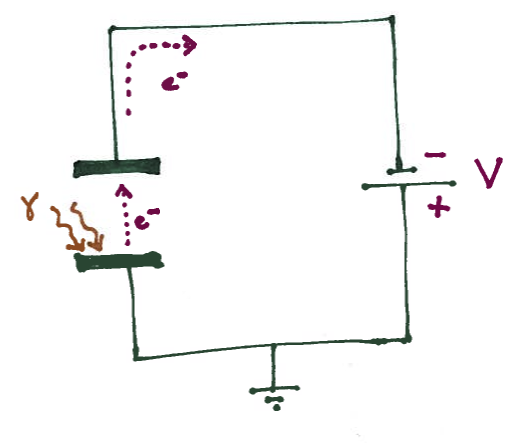
\includegraphics{circuito.png}
\caption{Arranjo t\'ipico do efeito fotoel\'etrico. Note que a luz indice sobre a placa inferior, chamada \textbf{anodo}, enquanto a placa superior, chamada \textbf{catodo}, coleta el\'etrons que conseguem se libertar do metal do anodo e est\~ao no v\'acuo entre as placas. Para mais detalhes veja texto.}
\end{figure}
A luz incide sobre a placa inferior. Se os f\'otons tiverem mais energia que a \textbf{fun\c c\~ao trabalho}, isto \'e, que a energia necess\'aria para liberar os el\'etrons da estrutura met\'alica, esse el\'etrons v\~ao escapar para o v\'acuo entre as placas, como representado pela seta pontilhada. Contudo, note que h\'a tamb\'em uma bateria no circuito. Essa bateria faz com que o fio na parte de cima esteja num potencial diferente do fio embaixo. Se assumirmos que o potencial do fio embaixo \'e 0, o potencial do fio de cima ser\'a negativo. Voc\^e pode dizer isso pela orienta\c c\~ao da baterial: veja que o terminal negativo (linha curta) est\'a ligada ao fio de cima.

Como el\'etrons s\~ao negativos e o potencial \'e negativo, os el\'etrons experimentam uma for\c ca contra seu movimento. Dito de outra forma, como tanta a carga do el\'etron quando o potencial el\'etrico \'e negativo, ent\~ao a energia potencial do fio em cima:

\begin{equation}
E_p = Q_E\times V > 0,
\end{equation}
\'e positiva. Num an\'alogo gravitacional, \'e como se houvesse uma montanha que os el\'etrons tem que subir e eles s\'o conseguem entrar no fio de cima se subirem essa montanha. Isto quer dizer que os el\'etrons tem que gastar essa energia potencial para conseguir se propagar no fio. Isso, claro, al\'em da energia gasta para se liberar da estrutura met\'alica (fun\c c\~ao trabalho). Desta forma, a energia cin\'etica do el\'etron \'e dada pela equ\c c\~ao \eqref{eq:energia}:
\begin{equation}
E_c = hf - \phi - Q_e\times V.
\end{equation}
A energia cin\'ética \'e um n\'umero maior ou igual a zero. Quando a energia cin\'etica dos el\'etrons \'e zero, isso quer dizer que n\~ao h\'a corrente el\'etrica (os el\'etrons n\~ao chegam no catodo). O potencial para o qual isso acontece \'e dado por:
\begin{equation}
0 = hf - \phi - Q_e\times V_{\text{max}}.
\end{equation}
Essa \'e uma maneira muito conveniente de se medir a fun\c c\~ao trabalho de um potencial. Dado que voc\^e sabe a freq\"u\^encia do f\'oton e o potencial da baterial em que a corrente cessa ($V_{\text{max}}$), a fun\c c\~ao taabalho pode ser encontrada resolvendo a equa\c c\~ao acima:
\begin{equation}
\phi = hf - Q_e\times V_{\text{max}}.
\end{equation}

\subsection{Sobre a energia cin\'etica dos el\'etrons}
Para entender a energia cin\'etica que os el\'etrons ter\~ao no circuito \'e importante primeiro entender a energia que eles tem enquanto est\~ao num s\'olido. Isso pode ser visto no diagrama da figura \ref{fig:bandas}. Sem a incid\^encia de luz, os el\'etrons com maior energia num metal estar\~ao na banda intermedi\'aria. Essa \'e a chamada banda de condu\c c\~ao. Isso quer dizer que eles podem se propagar livremente dentro do material (por isso que metais conduzem eletricidade), mas n\~ao podem escapar do material. A energia de el\'etrons livre \'e maior que el\'etrons de condu\c c\~ao e a diferen\c ca entre as duas bandas de energia \'e justamente a fun\c c\~ao trabalho que j\'a definimos acima.

\begin{figure}[ht]
\centering
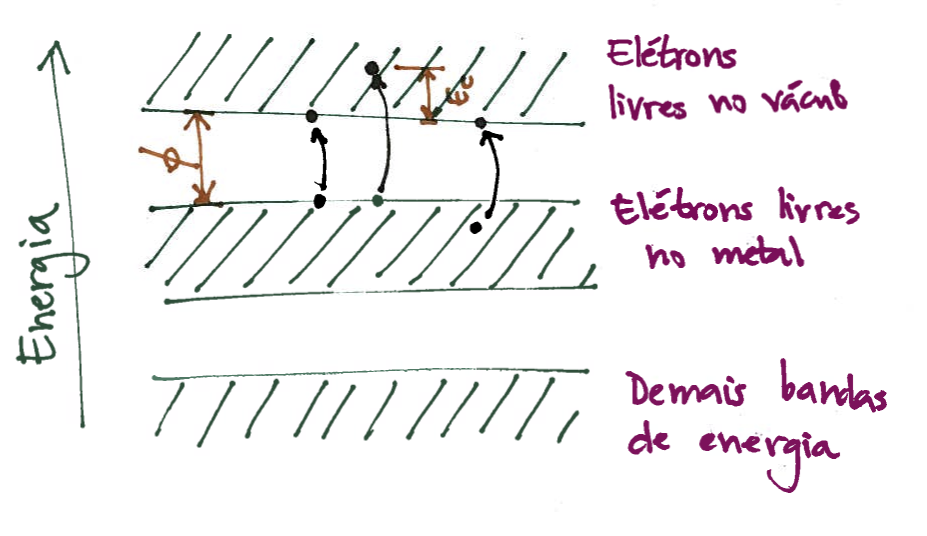
\includegraphics[width=0.9\textwidth]{bandas.png}
\caption{\label{fig:bandas}Estrutura de energia em bandas de um el\'etron num s\'olido. A figura mostra a chamada \textbf{banda de condu\c c\~ao}, na qual os el\'etrons podem se propagar livremente dentro do material e a diferen\c ca de energia $\phi$ para que os el\'etrons escapem do estrutura do material e possam se propagar livremente no v\'acuo fora do material. A diferen\c ca de energia entre essas duas bandas de energia \'e chamada \textbf{fun\c c\~ao trabalho} $\phi$.}
\end{figure}
Note que s\'olidos s\~ao essencialmente diferente de \'atomos livres. Em \'atomos livres (como num g\'as), os el\'etrons s\'o podem ter energias discretas bem definidas. Em s\'olidos eles podem ter \textbf{qualquer energia} em \textbf{bandas de energias}. Ent\~ao podemos imaginar diversas situa\c c\~oes distintas para como o efeito fotoel\'etrico ocorre no metal. Os tr\^es casos que quero discutir s\~ao representados pelas tr\^es setas escuras.

No primeiro caso (mais a esquerda), o el\'etron absorve um f\'oton que tem energia \textbf{exatamente} igual a fun\c c\~ao trabalho. Isso quer dizer que o el\'etron s\'o vai sair do material se ele tiver a maior energia poss\'ivel na banda de condu\c c\~ao. Se a energia dele fosse um poquinho menor, ele n\~ao escaparia. E, mesmo quando escapa, ele fica livre, mas parado, pois n\~ao sobra nenhuma energia como energia cin\'etica.

Nos dois outros casos o f\'oton tem mais energia que a fun\c c\~ao trabalho. Ent\~ao duas coisas podem acontecer. Esse f\'oton pode ser absorvido por um el\'etron na borda da banda de condu\c c\~ao, isto \'e, com a maior energia poss\'ivel dentro do material. Neste caso, o el\'etron se libera e ainda ter\'a uma energia cin\'etica $E_c$. Mas tamb\'em pode acontecer do f\'oton ser absrovido por um el\'etron com um pouco menos de energia (mais a direita na figura). Neste caso ele se liberar\'a, mas sua energia cin\'etica depois disso ser\'a zero.

A id\'eia que quero passar aqui \'e que a energia cin\'etica que escrevemos na f\'ormula \eqref{eq:energia}, n\~ao vai ser a energia cin\'etica de \textbf{todo} el\'etron liberado, mas sim a maior energia poss\'ivel. Alguns el\'etrons tinha uma energia menor dentro do material. Logo, algumas vezes voc\^e vai ver escrito:

\begin{equation}
E_c^{\text{max}} = hf - \phi - E_p.
\end{equation}

\section{Bremsstrahlung}

O proceso de bremsstrahlung tem os seguintes estados iniciais e finais:

\begin{equation}
\text{el\'etron livre} \rightarrow \text{el\'etron livre} + \text{f\'oton}.
\end{equation}
A palavra bremsstrahlung vem do alem\~ao e significa, literalmente, energia de frenamento. Isso porque o el\'etron \'e desacelerado durante o processo. Em outras palavras, o el\'etron livre do estado final tem uma energia cin\'etica maior que a o el\'etron no estado final. A diferen\c ca entre as duas energias \'e a energia do f\'oton. Logo, a freq\"u\^encia, $f$, do f\'oton emitida \'e:

\begin{equation}\label{eq:energia2}
f = \frac{E_c(\text{el\'etron final})-E_c(\text{el\'etron inicial})}{h}
\end{equation}

Essa \'e uma das formas mais comuns de se produzir raio X. As m\'aquinas de raio X em hospitais, por exemplo, usam exatamente esse m\'etodo. Aqui estamos assumindo duas coisas:

\begin{enumerate}
\item O el\'etron perde toda sua energia cin\'etica.
\item Toda a energia \'e transferida para apenas um f\'oton.
\end{enumerate}
Ambas hip\'oteses n\~ao s\~ao necessiaramente verdade. O el\'etron perde sua energia interagindo com algum material, vamos supor que esse material \'e exposso o suficiente para parar o el\'etron. Isto \'e, o caso (1) acima n\~ao nos interessa aqui. No segundo caso, o el\'etron pode emitir diversos f\'otons tal que a soma de todas as energias emitidas \'e igual a sua energia inicial. Nesse caso cada f\'oton individual ter\'a uma frequ\"u\^encia (e, logo, energia) menor do que aquela escrita em \eqref{eq:energia2}.
\end{document}
